\author{Daniel De Lucca Fonseca}

\documentclass[11pt]{article}
\usepackage{float}
\usepackage{url}
\usepackage{epsfig}
\usepackage[brazil, english]{babel}
\usepackage[utf8]{inputenc}    
\usepackage{csquotes}
\usepackage{multirow}
\usepackage{hyperref}
\usepackage{color}
\usepackage{verbatim}
\usepackage{acronym}
\usepackage[style=ieee]{biblatex}
\usepackage{graphicx}
\graphicspath{{images/}}
\usepackage{booktabs}
\usepackage{caption} 
\captionsetup[table]{skip=10pt}

\addbibresource{main.bib}
\input{chapters/i-acronyms.tex}

\special{papersize=8.5in,11in}
\setlength{\textwidth}{6.5in} \setlength{\textheight}{9.0in}

\setlength{\evensidemargin}{-.2in}
\setlength{\oddsidemargin}{0.0in} \setlength{\topmargin}{-.4in}
\setlength{\topmargin}{-.4in}
\linespread{1.5}

\begin{document}
%  ABACO -- Conjunto de macros para desenhar o 'abaco

%  Desenho original de Hans Liesenberg

%  Macros de Tomasz Kowaltowski

%  DCC -- IMECC -- UNICAMP

%  Mar,co de 1988  --  Vers~ao 1.0

% Ajustado para LaTeX da SUN -- Mar,co de 1991

% ---------------------------------------------------------

%  Chamada:   \ABACO{d1}{d2}{d3}{d4}{esc}
%             com:  di's -- os quatro d'igitos;
%	           esc  -- fator de escala

% ---------------------------------------------------------

%  DEFINI,C~OES AUXILIARES

% ---------------------------------------------------------


%  Forma o d'igito pequeno (0 ou 1)

\newcommand{\ABACODP}[1]{%
%
\thicklines
%    
\begin{picture}(8,0)
    \ifcase#1{   %  caso 0
       \put(0,0)    {\line(1,0){4}}
       \multiput(5,0)(2,0){2}{\oval(2,4)}}
    \or{         %  caso 1
       \put(2,0)    {\line(1,0){4}}
       \multiput(1,0)(6,0){2}{\oval(2,4)}}
    \fi
\end{picture}
    } % \ABACODP

% Forma o d'igito grande (0 a 4)

\newcommand{\ABACODG}[1]{%
%
\thicklines
%    
\begin{picture}(14,0)
    \ifcase#1{   % caso 0
       \multiput(1,0)(2,0){5}{\oval(2,4)}}
       \put(10,0)   {\line(1,0){4}}
    \or{         % caso 1
       \multiput(1,0)(2,0){4}{\oval(2,4)}}
       \put(8,0)   {\line(1,0){4}}
       \put(13,0)   {\oval(2,4)}
    \or{         % caso 2
       \multiput(1,0)(2,0){3}{\oval(2,4)}
       \put(6,0)   {\line(1,0){4}}
       \multiput(11,0)(2,0){2}{\oval(2,4)}}
    \or{         % caso 3
       \multiput(1,0)(2,0){2}{\oval(2,4)}
       \put(4,0)   {\line(1,0){4}}
       \multiput(9,0)(2,0){3}{\oval(2,4)}}
    \or{         % caso 4
       \put(1,0)  {\oval(2,4)}}
       \put(2,0)   {\line(1,0){4}}
       \multiput(7,0)(2,0){4}{\oval(2,4)}
    \fi
\end{picture}
    } % \ABACODG
       
% Forma um d'igito (0 a 9)

\newcommand{\ABACOD}[1]{%
%
    \ifnum#1>9
       \errmessage{#1: Argumento invalido para ABACO}
    \fi
    \ifnum#1<0
       \errmessage{#1: Argumento invalido para ABACO}
    \fi
%
\begin{picture}(24,0)
%    
    \ifnum#1<5
       \put(16,0) {\ABACODP{0}}
    \else   
       \put(16,0) {\ABACODP{1}}
    \fi
%    
    \ifnum#1<5
       \put(0,0)  {\ABACODG{#1}}
    \else
       \ifcase#1\or \or \or \or
          \or  \put(0,0)  {\ABACODG{0}}
          \or  \put(0,0)  {\ABACODG{1}}
          \or  \put(0,0)  {\ABACODG{2}}
          \or  \put(0,0)  {\ABACODG{3}}
          \or  \put(0,0)  {\ABACODG{4}}
       \fi
    \fi   
\end{picture}
    } % \ABACOD
    
% -------------------------------------------------

%  DEFINI,C~AO PRINCIPAL
    
\newcommand{\ABACO}[5]{%
    \setlength{\unitlength}{#5mm}
%
    \thinlines
%   
\begin{picture}(28,25)
%   
% moldura
%
% externa
%
        \put(0,0)            {\line(0,1){25}}
        \put(0,0)            {\line(1,0){28}}
        \put(28,0)           {\line(0,1){25}}
        \put(0,25)           {\line(1,0){28}}
% interna
        \put(2,2)            {\line(0,1){21}}
	\put(26,2)           {\line(0,1){21}}
	\put(16,2)           {\line(0,1){21}}
	\put(18,2)           {\line(0,1){21}}
	\put(2,2)            {\line(1,0){14}}
	\put(16,2)           {\line(1,-1){1}}
	\put(17,1)           {\line(1,1){1}}
	\put(18,2)           {\line(1,0){8}}
	\put(2,23)           {\line(1,0){14}}
	\put(16,23)          {\line(1,1){1}}
	\put(17,24)          {\line(1,-1){1}}
	\put(18,23)          {\line(1,0){8}}
	\put(0,0)            {\line(1,1){2}}
	\put(0,25)           {\line(1,-1){2}}
	\put(28,0)           {\line(-1,1){2}}
	\put(28,25)          {\line(-1,-1){2}}
%
%   
% d'igitos
%
%   
       \put(2,20)  {\ABACOD{#1}}
       \put(2,15)  {\ABACOD{#2}}
       \put(2,10)  {\ABACOD{#3}}
       \put(2,5)   {\ABACOD{#4}}
%      
\end{picture}
    } % \ABACO
    


\begin{titlepage} 

    \begin{center} 
        \large \textbf{UNIVERSITY OF CAMPINAS}\\
        \large INSTITUTE OF COMPUTING\\
        
        \vspace{0.5cm}

        \begin{minipage}[tl]{31mm}
            \ABACO{1}{9}{6}{9}{1}
        \end{minipage}

        \vspace{0.3cm}
        \textbf{Dwsr: Predicting the memory usage of tensorial algorithms}
        \vspace{0.2cm}

        \begin{tabular}{rl}
            \textbf{Student}: & Daniel De Lucca Fonseca \\
            \textbf{Advisor}: & Prof. Edson Borin \\
        \end{tabular}

    \end{center}

\textbf{Abstract:} Lorem ipsum dolor

\end{titlepage} 

%----------------MACROS-----------------------------------------

\newcommand{\EB}[1]{{\bf \textcolor{red}{(EB: #1)}}}
\newcommand{\EBH}[1]{\hl{#1}}
\newcommand{\EBC}[2]{\EBH{#1} \EB{#2}}
\newcommand{\EBADD}[1]{{\textcolor{red}{#1}}}
\newcommand{\EBRM}[1]{{\textcolor{lightgray}{(#1)}}}
\newcommand{\EBRP}[2]{\EBRM{#1}\EBADD{#2}}
\newcommand{\EBRPD}[2]{#1 \EB{#1 $\rightarrow$ #2?}}

\newcommand{\DF}[1]{{\bf \textcolor{blue}{(DF: #1)}}}
\newcommand{\DFH}[1]{\hl{#1}}
\newcommand{\DFC}[2]{\DFH{#1} \DF{#2}}
\newcommand{\DFADD}[1]{{\textcolor{blue}{#1}}}
\newcommand{\DFRM}[1]{{\textcolor{lightgray}{(#1)}}}
\newcommand{\DFRP}[2]{\DFRM{#1}\DFADD{#2}}
\newcommand{\DFRPD}[2]{#1 \DF{#1 $\rightarrow$ #2?}}


%----------------CONTENT TABLE----------------------------------
\setlength{\baselineskip}{0.1 cm}
\pagenumbering{roman} \pagebreak
\normalsize \tableofcontents \pagebreak
\pagenumbering{arabic}

\acresetall

%---------------CHAPTERS---------------------------------------
\section{Introduction}
\label{sec:introduction}

Memory management is a crucial aspect of modern computer applications.
Some problems, such as seismic processing, are particularly sensitive to the amount of available memory.
Due to the large size of seismic data, even the most powerful supercomputers cannot execute a computing graph in a single node.
To overcome this challenge, most seismic algorithms rely on data parallelism.

For some algorithms, choosing the right data partitioning strategy is quite straightforward.
On the other hand, the optimal strategy isn't so obvious for others, usually because they require a large amount of work memory.
The latter is true for some seismic processing algorithms, therefore the data partitioning strategy is usually defined after a series of trials and errors.
Although this approach is effective, it is time consuming and requires a lot of human effort.

In this research proposal, I suggest exploring about a new ata partitioning strategy for data parallelism.
The proposed strategy is based on the \emph{memory footprint} of the algorithm, which is the amount of memory required to execute it.
This approach may be effective not only for seismic algorithms, but also for any other algorithm that has a predictable memory footprint.
The process is divided into two main stages:
(i) the \emph{memory footprint estimation} stage, where the memory footprint of the algorithm is estimated; and
(ii) the \emph{data partitioning} stage, where the data is partitioned according to the estimated memory footprint.

For the memory footprint estimation stage, I propose to use a machine learning model to predict the memory footprint of the algorithm.
Most of the existing research to predict the memory footprint of an algorithm focus on predicting resource consumption from a scheduler's perspective, while no research has been conducted to predict it for a single algorithm.

For the data partitioning stage, I propose to leverage DASK~\cite{dask} automatic chunking to partition the data.
DASK is a Python library that provides a high-level interface to parallelize Python code.
Considering that we can estimate the memory usage, figuring out the optimal chunk size is a matter of finding the relationship between the amount of available memory and the memory footprint itself.

During this research, I am planning to work with DASF~\cite{dasf} to implement the proposed strategy.
DASF is a library created by the Discovery laboratory at UNICAMP to facilitate the development of seismic processing algorithms.

The following sections are organized as follows.
I start by presenting the background on section~\ref{sec:background}, explaining relevant concepts for this research.
Then, I present the related work on section~\ref{sec:related-work}, where I discuss the existing research on memory usage estimation and resource-aware scheduling.
Finally, I present the research proposal on section~\ref{sec:research-proposal}, where I describe the research plan and the expected results.

\section{Background}
\label{sec:background}

This section presents and discusses all relevant background knowledge needed to understand the rest of the proposal.
Each subsection will present a specific topic, giving a general overview and discussing its relevance to the project.

\subsection{Seismic attributes}
\label{subsec:seismic-attributes}

Seismic attributes are quantitative measures derived from seismic data, which describe various aspects of the subsurface geology.
Over the past few decades, seismic attributes have become an indispensable tool in the exploration and production of hydrocarbons, mineral resources, and the management of geohazards.
They have significantly contributed to the understanding of complex geological settings and have improved the accuracy of reservoir characterization and prediction.

Seismic data, which is obtained through the use of controlled seismic sources and an array of receivers, is used to create images of the subsurface geology.
The acquired data is processed and interpreted to reveal geological features, such as faults, fractures, and rock properties.
However, seismic data can be challenging to interpret due to the complex nature of the subsurface geology and the limitations of seismic imaging techniques.

The evolution of seismic attributes is explored in Barnes and Arthur~\cite{barnes2001seismic}, Chopra \emph{et al.}~\cite{chopra2005seismic}, Fawad \emph{et al.}~\cite{fawad2020seismic}, and Taner and Turhan~\cite{taner2001seismic}.
This concept was first introduced in the late 1970s as a means to enhance the interpretation of seismic data.
Since then, the field has experienced significant advancements, driven by the growth in computational power and the development of innovative seismic processing and interpretation techniques.
Seismic attributes can be broadly classified into five categories:

\begin{itemize}
    \item \textbf{Amplitude-based attributes}: These attributes are derived from the amplitude of the seismic waveforms and are used to analyze variations in rock properties, fluid content, and stratigraphy.
        Common examples of amplitude-based attributes include average amplitude, root-mean-square amplitude, and instantaneous amplitude;
    \item \textbf{Frequency-based attributes:} These attributes focus on the frequency content of the seismic data and can reveal information about the thickness and composition of subsurface layers.
        Examples of frequency-based attributes include spectral decomposition, dominant frequency, and instantaneous frequency;
    \item \textbf{Time and spatial-based attributes:} These attributes describe the geometrical and temporal properties of seismic events, such as the continuity, dip, and azimuth of reflectors.
        Some examples of time and spatial-based attributes are coherence, curvature, and semblance;
    \item \textbf{Mitigation attributes:} These attributes are designed to reduce the impact of noise and other artifacts in the seismic data, improving the overall quality and interpretability of the data.
        Examples of mitigation attributes include random noise attenuation, multiple suppression, and ground roll removal;
    \item \textbf{Texture attributes:} These attributes characterize the texture or patterns within the seismic data, providing insights into geological features such as fractures, channels, and stratigraphic boundaries.
        Texture attributes can be computed using techniques such as gray-level co-occurrence matrices, wavelet decomposition, and local binary patterns.
\end{itemize}

To illustrate how seismic attributes are used, figure~\ref{fig:seismic-complex-attr} shows a sample of two complex seismic attributes derived from the amplitude of a sample seismic data.
The envelope of the amplitude, which is ilustrated by figure~\ref{fig:seismic-envelope}, highlights the presence of a possible hydrocarbons reservoir.
Figure~\ref{fig:seismic-inst-phase} shows the instantaneous phase of the seismic data, which defines the phase of the seismic wavelet at each sample.

\begin{figure}[htb!]
    \captionsetup[subfigure]{justification=centering}
    \centering

    \subfloat[][Amplitude (raw data)]{
        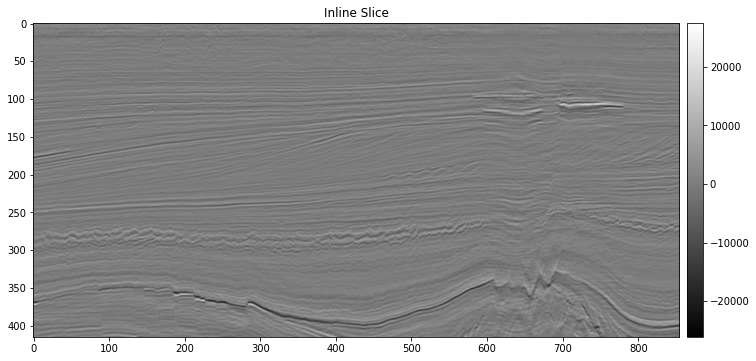
\includegraphics[height=4cm]{images/seismic-amplitude.png}
        \label{fig:seismic-raw-data}
    }
    
    \subfloat[][Amplitude envelope (the red arrow highlights a possible hydrocarbons reservoir)]{
        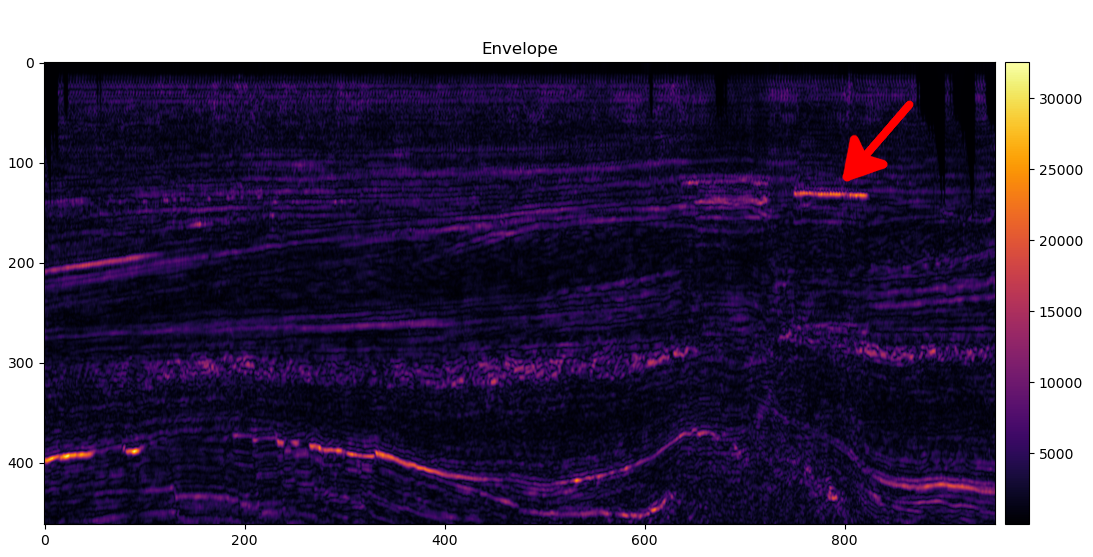
\includegraphics[height=4cm]{images/seismic-envelope.png}
        \label{fig:seismic-envelope}
    }
    \subfloat[][Instantaneous phase]{
        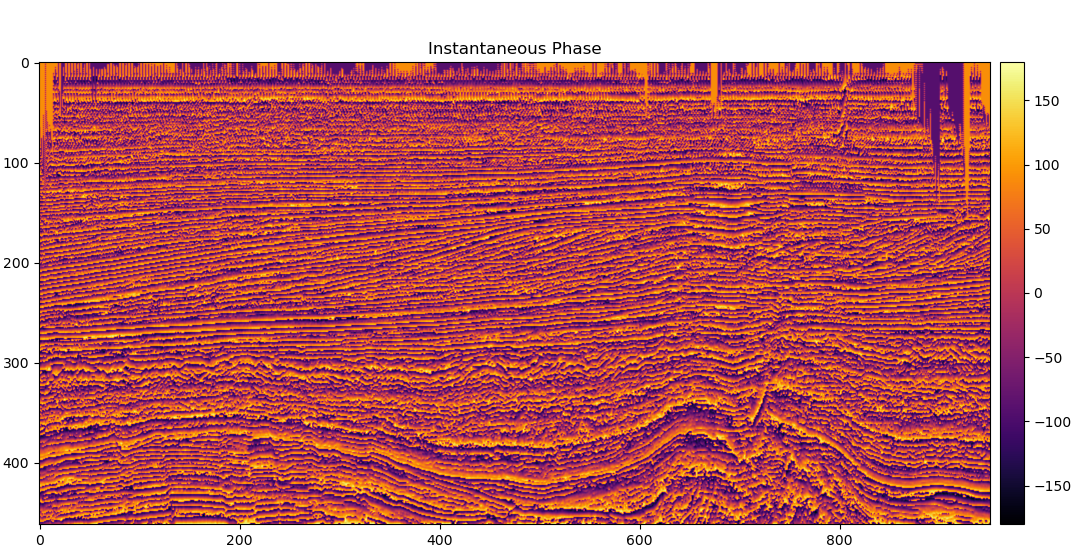
\includegraphics[height=4cm]{images/seismic-inst-phase.png}
        \label{fig:seismic-inst-phase}
    }

    \caption{Sample of two complex seismic attributes derived from the amplitude to the inline}
    \label{fig:seismic-complex-attr}
\end{figure}

As explained in the previous example, the integration of seismic attributes into the interpretation workflow allows geoscientists to extract valuable information from seismic data more efficiently.
Seismic attributes can be combined with other data, such as well logs and geological models, to provide a comprehensive understanding of the subsurface geology.
Furthermore, advanced machine learning and data analytics techniques have enabled the development of multi-attribute analysis, which involves the simultaneous examination of multiple attributes to identify patterns and relationships that may not be apparent when considering individual attributes.

In summary, seismic attributes play a crucial role in the analysis and interpretation of seismic data by providing quantitative measures of subsurface geology.
They enhance the understanding of complex geological settings, improve reservoir characterization, and aid in the prediction of subsurface resources.
As the field continues to evolve, the integration of seismic attributes with other data sources and advanced computational techniques will further advance the state of knowledge in the field and enable more accurate and efficient exploration and production efforts.

\subsection{Memory footprint}
\label{subsec:memory-footprint}

The memory footprint of an algorithm refers to the amount of memory space required for its execution, considering both static and dynamic memory allocations.
It is a crucial performance metric, as it directly affects the overall system resources and impacts the efficiency and scalability of an algorithm.
In essence, the memory footprint is an essential aspect of an algorithm's resource consumption, alongside other factors such as time complexity and processing power.

\emph{Static memory allocation} is the memory allocated during compile-time, which includes the memory needed for storing executable code, global variables, and static local variables.
This memory remains fixed throughout the program's execution and is typically allocated in the text, data, and \ac{BSS} segments.

On the other hand, \emph{dynamic memory allocation} refers to the memory allocated during run-time, including the memory needed for storing dynamically allocated variables, function call stacks, and memory required by recursive functions.
This type of memory allocation occurs in the heap and stack segments.

To achieve a deeper understanding of the memory footprint of an algorithm, it is possible to evaluate the following components:

\begin{itemize}
    \item \emph{Space Complexity:} Measures the total amount of memory an algorithm uses as a function of its input size.
        This evaluation usually uses the big-O notation, such as $O(n)$ or $O(n^2)$, where $n$ is the input size.
        It is possible to split space complexity into two subtypes:
        (i) auxiliary space (temporary memory used during execution) and
        (ii) input space (memory needed for storing input data);
    \item \emph{Data Structures:} An algorithm's choice of data structures significantly influences its memory footprint.
        Different data structures have varying memory overheads and trade-offs, and selecting the most appropriate data structure can lead to substantial improvements in memory usage;
    \item \emph{Memory Management Techniques:} The way an algorithm manages memory can substantially impact its memory footprint.
        This includes memory allocation and deallocation strategies, garbage collection, and other techniques that optimize memory usage during the algorithm's execution.
\end{itemize}

The memory footprint of an algorithm is a critical aspect of its performance, as it directly influences the overall system resources and efficiency.
By comprehending and optimizing the memory footprint of an algorithm, developers can create more efficient and scalable solutions, ultimately contributing to improved computational capabilities in various applications and industries.

\subsection{Dask}
\label{subsec:dask}

Dask~\cite{dask} is a powerful and flexible parallel computing framework designed for the Python ecosystem.
It enables users to harness the power of parallel and distributed computing to scale their applications and data processing tasks.
Dask~\cite{dask} was created to address the limitations of traditional Python libraries like NumPy~\cite{numpy} and Pandas~\cite{pandas}, which struggle to handle large-scale datasets due to their in-memory computation model.
It addresses these limitations by providing parallelized and out-of-core computation capabilities.

Dask~\cite{dask} works by breaking down large-scale tasks into smaller, manageable tasks that can be executed in parallel across multiple cores or even distributed across multiple machines.
It builds a task graph, which is a visual representation of the tasks and their dependencies, allowing for efficient scheduling and execution of tasks.
Dask~\cite{dask} can automatically manage and distribute these tasks, making it easier for users to scale their applications.

Some of the key features of Dask~\cite{dask} are:
(i) parallelism that can leverage the available hardware resources,
(ii) out-of-core computation, which allows handling datasets that are too large to fit into memory,
(iii) dynamic task scheduling, and
(iv) Integration with existing Python libraries.

Code sample~\ref{lst:dask-sample-001} shows an example of how Dask~\cite{dask} can be used to parallelize NumPy~\cite{numpy} operations, while code sample~\ref{lst:dask-sample-002} shows how Dask~\cite{dask} can be used to parallelize Pandas~\cite{pandas} operations.

\lstinputlisting[language=Python, caption=Parallelizing NumPy~\cite{numpy} operations, label=lst:dask-sample-001]{code/dask-sample-001.py}
\lstinputlisting[language=Python, caption=Parallelizing Pandas~\cite{pandas} operations, label=lst:dask-sample-002]{code/dask-sample-002.py}

\subsection{Reinforcement Learning}
\label{subsec:reinforcement-learning}

Reinforcement learning is a branch of machine learning that focuses on training intelligent agents to make decisions based on the consequences of their actions in a given environment~\cite{kaelbling1996}.
It has emerged as a powerful method for solving complex problems in various fields.

In reinforcement learning, the model, known as an agent, interacts with an environment to learn an optimal policy for achieving its goals.
The agent selects actions based on their current state and receives feedback from the environment through rewards or penalties.
This feedback guides the agent's learning process, allowing it to improve its decision-making abilities over time.

The central components of a reinforcement learning system include:

\begin{itemize}
    \item \emph{Agent:} The intelligent entity that learns and makes decisions based on its interactions with the environment;
    \item \emph{Environment:} The context or world within which the agent operates, offering various states, actions, and feedback;
    \item \emph{State:} The representation of the agent's current situation within the environment;
    \item \emph{Action:} The possible moves or decisions the agent can make within the environment;
    \item \emph{Reward:} The feedback the environment provides indicates the success or failure of an agent's actions.
\end{itemize}

Reinforcement learning algorithms can be broadly categorized into model-free and model-based methods, as well as on and off-policy methods:

On \emph{model-free methods}, the agent learns directly from its interactions with the environment without knowing the underlying dynamics.
The agent learns to map states to actions based on trial and error.
Examples of model-free methods include Q-learning~\cite{watkins1992}, SARSA~\cite{rummery1994}, and \ac{DQNs}~\cite{mnih2015}.
On the other hand, on \emph{model-based methods}, the agent learns a model of the environment, which captures the dynamics of state transitions and rewards.
This model is then used to plan and select optimal actions.
Techniques employed in model-based methods include Monte Carlo Tree Search~\cite{browne2012}, Dynamic Programming, and various planning algorithms.

Regarding policy methods, \emph{on-policy methods} involve the agent learning the value of its current policy while following it.
The agent continually updates its policy based on the experience gained through its actions.
On-policy algorithms include SARSA~\cite{rummery1994}, which learns the action-value function for the current policy, and actor-critic methods that learn both a value function and a policy.
In contrast to on-policy methods, \emph{off-policy methods} enable the agent to learn the optimal policy while following another policy.
This approach provides more flexibility, as the agent can learn from the experiences of other agents or explore different policies simultaneously.
Q-learning~\cite{watkins1992} and \ac{DDPG}~\cite{wang2022} are examples of off-policy algorithms.

According to Sutton and Barto~\cite{sutton1998}, the critical steps for the process of reinforcement learning are:
(i) initialization, when the agent starts in an initial state and initializes its learning parameters, such as the action-value function or policy;
(ii) action selection, when the agent chooses an action based on its current policy or action-value function, often incorporating exploration strategies like epsilon-greedy or softmax action selection;
(iii) environment interaction, when the agent performs the chosen action, and the environment responds by providing a reward and transitioning to a new state;
(iv) learning, when the agent updates its knowledge based on the experience gained from the interaction, adjusting its policy or action-value function;
(v) repetition, steps ii through iv are repeated until a termination condition is met, such as reaching a maximum number of steps, achieving a certain level of performance, or converging on an optimal policy.

Despite the promising capabilities of reinforcement learning, challenges and limitations exist, such as exploration vs. exploitation trade-offs, sparse rewards, and sample efficiency.
Balancing exploration (trying new actions) with exploitation (selecting known optimal actions) is crucial for an agent to learn effectively.
Additionally, agents must learn to cope with environments where rewards are infrequent or delayed, which can slow down the learning process.

Another challenge in reinforcement learning is dealing with the curse of dimensionality~\cite{weber1998}.
As the state and action spaces become more complex, the time and computational resources required for learning can grow exponentially.
Researchers have developed various techniques to tackle this issue, such as function approximation, state aggregation, and hierarchical reinforcement learning.

Reinforcement learning offers a robust framework for training intelligent agents to make decisions in complex environments.
Despite the challenges and limitations, ongoing research pushes the boundaries of what reinforcement learning can achieve, paving the way for its application in various fields and real-world problems.


\section{Related Work}
\label{sec:related-work}

This section will discuss the existing research related to this proposal.
Most existing work aiming to predict memory consumption focuses on \emph{resource-aware scheduling}.
The most common use case for this research type is to predict memory consumption to allocate resources in a cluster efficiently.
There are a few works that focus on \emph{resource-aware execution}, most of those focused entirely on some particular use cases.

This section compares and contrasts the current state-of-the-art of each existing approach, evaluating the main differences between the proposed work and the existing research.
Finally, by the end of this section, table~\ref{tab:related-work-comparison} summarises the main findings.

\subsection{Resource-aware scheduling}
\label{subsec:resource-aware-scheduling}

Pupykina et al.~\cite{pupykina2019} presets a nice overview of the memory management field until 2019.
According to the authors, the main challenge on predicting memory usage is the lack of knowledge of the memory access patterns within an application.
Most of current research focus on using machine learning techniques to bypass this problem.
Although this approach has been successful, it is only capable of predicting the overall resource usage of a whole workload, and not the resource usage of a single task.

The observation made by Pupykina et al.~\cite{pupykina2019} is visible while evaluating recent work.
Most of the research done so far focus only on the scheduler perspective, using memory usage history to predict the expected resource requirements of a given cluster.

E. R. Rodrigues et al.~\cite{rodrigues2016} presents a machine learning model that can easily be integrated into a scheduler to predict the resource requirements of a given task.
Their work is mainly focused on the scheduler perspective, since it uses past executions by the user to predict the resource requirements for future jobs.
While submiting a new job to the cluster, the user must provide a manual estimate.
This estimate is used by E. R. Rodrigues et al.~\cite{rodrigues2016} alongside with past executions to predict the actual resource requirements of the job.
Although effective, this approach is vulnerable to spurious correlations, since past executions from other jobs by the same user can influence the prediction.

T. Mehmood et al.~\cite{mehmood2018} presents an ensemble machine learning model that can predict the expected resource usage of a cloud provider.
Like E. R. Rodrigues et al.~\cite{rodrigues2016}, T. Mehmood et al.~\cite{mehmood2018} uses past executions to predict the resource requirements at a given time.

% Althoug 
% B. T. Shealy et al.~\cite{shealy2021} presents a machine learning model that can consider both the memory usage history, as well as which run command flags were used to execute a given task, to predict the resource requirements of a given task.
% Their work is mainly focused on recurrent tasks, 

\subsection{Resource-aware execution}
\label{subsec:resource-aware-execution}

D. Duplyakin \emph{et al.}~\cite{duplyakin2018} takes a different approach to evaluate the resource usage of a given algorithm.
Instead of using the execution history in order to predict the expected requirements to efficiently handle resource allocation, D. Duplyakin \emph{et al.}~\cite{duplyakin2018} tries to incrementally model the memory usage of the algorithm using an active learning approach.
Their discovery is important, since they successfully demonstrated that it is possible to integrate active learning with gaussian process regression in order to explore the resource usage of a given algorithm.
However, their approach is tighly coupled to their use-case, but the same concept can be explored on a more general approach.

Following a similar perspective, C. Tang \emph{et al.}~\cite{tang2021} proposes a method to predict the resource usage of a given query.
Their approach was developed inside Twitter~\footnote{https://twitter.com/}, and aims to simplify the calculation of the resource usage of SQL queries.
During their research, C. Tang \emph{et al.}~\cite{tang2021} were able to extract keywords and features directly from the query itself and use those features to increase the prediction accuracy.
With that method, they were able to achieve an average accuracy of 97\%.
Considering this, their research demonstrated that it is possible to use the source code of a given algorithm to predict its resource usage.
Although their context is limited to SQL queries, the same concept can be generalized to other programming languages.

As demonstrated by D. Duplyakin \emph{et al.}~\cite{duplyakin2018} and C. Tang \emph{et al.}~\cite{tang2021}, it is possible to predict the resource usage of a single algorithm both by exploring key aspects of the application, as well as by dynamically exploring unknown executions.
However, both approaches are limited to a specific use-case, and they do not provide a general solution to predict the resource usage of any given algorithm.


\aboverulesep = 0mm
\belowrulesep = 0mm

\begin{table}[ht]
  \caption{Related work comparison table}
  \label{tab:related-work-comparison}
  \resizebox{\textwidth}{!}{%
    \begin{tabular}{@{}|p{0.11\linewidth}|p{0.3\linewidth}|p{0.5\linewidth}|p{0.3\linewidth}|p{0.3\linewidth}|p{0.2\linewidth}|@{}}
      \toprule
      \textbf{Work}        & \textbf{Model strategy}                                       & \textbf{Used features}                                                                                  & \textbf{Prerequisites}                          & \textbf{Purpose}              & \textbf{Perspective}  \\ \midrule
      \cite{rodrigues2016} & Poll of machine learning models specialized per cluster       & Memory usage, user metadata, and job metadata                                                           & Cluster management software and past executions & Scheduler resource allocation  & Scheduler            \\ \midrule
      \cite{mehmood2018}   & Ensemble-based machine learning model specialized per cluster & Resource usage history                                                                                  & Resource usage traces                           & Scheduler resource allocation  & Scheduler            \\ \midrule
      \cite{phung2021}     & Heuristic-based generic model                                 & Resources being used and user-provided information                                                      & User information about the task                 & Scheduler resource allocation  & Scheduler            \\ \midrule
      \cite{fang2018}      & Least squares-based generic model                             & Resources being used and memory pressure                                                                & Resource competition                            & Scheduler resource allocation  & Scheduler            \\ \midrule
      \cite{ferreira2013}  & \ac{MAPE-K} specialized per task                              & Input data parameters                                                                                   & Manual profiling                                & Efficient task scheduling      & Scheduler            \\ \midrule
      \cite{shealy2021}    & A single machine learning model per algorithm                 & Memory usage history, input structure, and run command flags                                            & Past executions and code instrumentation        & Recurrent task scheduling      & Scheduler            \\ \midrule
      \cite{goponenko2020} & Adaptive scheduling strategy per cluster                      & Memory usage estimate                                                                                   & Past executions                                 & Efficient task scheduling      & Scheduler            \\ \midrule
      \cite{duplyakin2018} & \ac{GPR} model specialized for \ac{AMR} simulations           & Hardware-specific data and simulation parameters                                                        & \ac{AMR} simulations and historical data        & Predict resource consumption   & Algorithm            \\ \midrule
      \cite{tang2021}      & Supervised learning specialized for a specific domain         & Memory usage history and executed query                                                                 & Query logs                                      & Query resource usage estimate  & Algorithm            \\ \midrule
      This work            & Reinforcement learning                                        & Input data shape and memory consumption                                                                 & None                                            & Parallelism optimization       & Graph                \\ \midrule
    \end{tabular}
  }
\end{table}

\section{Research proposal}
\label{sec:research-proposal}

In this research proposal, we aim to predict computer memory consumption from an algorithmic perspective.
While there have been numerous studies on memory usage history analysis from the scheduler perspective, we believe that there is a significant gap in research when it comes to predicting memory usage of a specific algorithm.

\subsection{Problem statement}
\label{subsec:problem-statement}

The Discovery~\footnote{\url{https://discovery.ic.unicamp.br/}} laboratory, located at \ac{UNICAMP}~\footnote{\url{https://ic.unicamp.br/}}, is working on a seismic analysis project with Petrobras~\footnote{\url{https://petrobras.com.br/}}.
This project relies heavily on machine learning and seismic operators for its computing graphs.
However, the input of these graphs is a massive seismic dataset that can contain terabytes of data.
Even supercomputers do not have enough memory to handle the computation on a single node.
Therefore, usually the execution is distributed by using data parallelism.

To facilitate this process, our laboratory implemented a framework called \ac{DASF}~\cite{dasf} that simplifies the development of data-parallel computing graphs using Dask~\cite{dask} under the hood.
\ac{DASF}~\cite{dasf} has an input parameter called \textbf{block\_size} that defines the size of each seismic block used during data parallelism.
However, setting this parameter can be challenging because it required finding the optimal relationship between it and the network overhead caused by it.

To illustrate this challenge, I present image~\ref{fig:block\_size} which contains three computing graphs receiving input data from a seismic dataset.
The first graph shows the input data as the entire dataset, which requires a significant amount of memory to execute.
The second graph divides the data into thousands of small parts, reducing the memory requirement but adding network overhead.
The third graph divides the data into a smaller number of parts, minimizing both network and memory requirements.

\begin{figure}[h]
\label{fig:block-size}
\caption{Block size impact on memory and network usage}
\resizebox{\textwidth}{!}{%
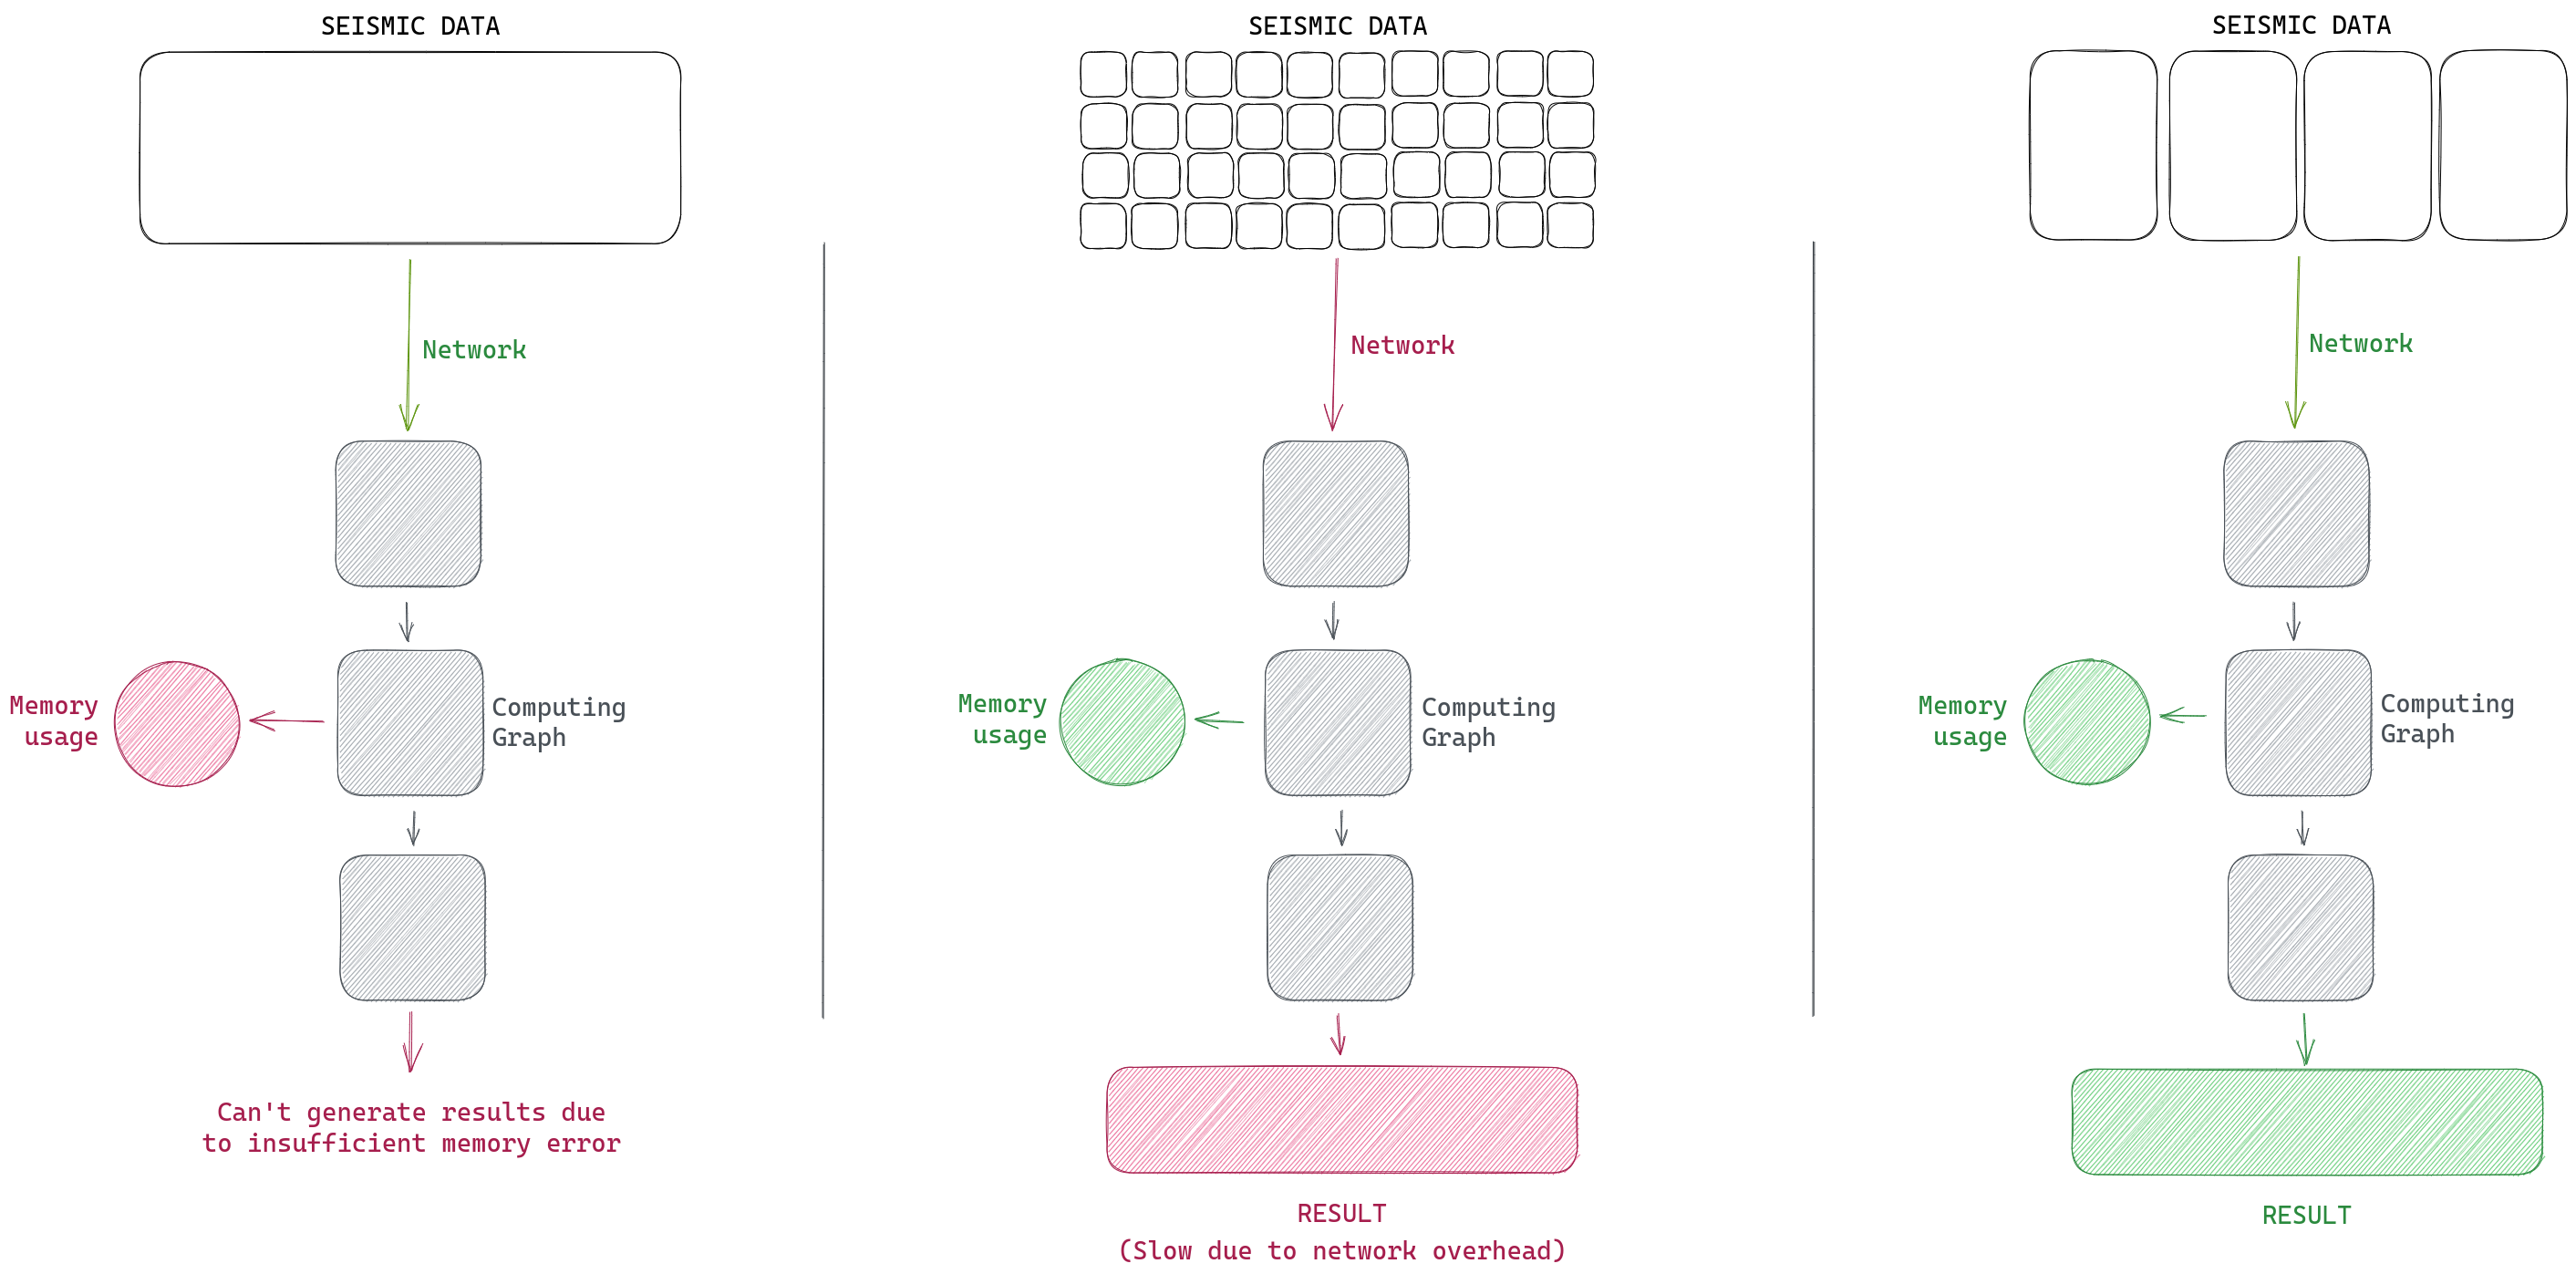
\includegraphics{block_size.png}
}
\end{figure}

While executing the graph, the developer must manually set the block\_size parameter.
Setting a large number may lead to memory issues and it causes a signifcant delay due the trial-and-error nature of the execution flow.
Since Petrobras uses supercomputers to execute those graphs, this delay is even larger considering the time it takes to submit a job due to the queue waiting time.

On the other hand, setting a small number may increase the execution time due to network overhead.
Since Petrobras have a large number of graphs to execute, and each graph usually takes a long time to execute, I need to find a way to optimize the block\_size parameter.

Dask~\cite{dask} provides an automatic chunking feature, but it relies on the chunk\_size parameter, which is a static parameter define prior to execution.
Since the developer do need to define this parameter prior to the execution, they can't rely on Dask~\cite{dask} auto chunking feature to automatically split the data, but they can rely on the automatic chunking if they figure out the ideal chunk\_size prior to the execution.

Figuring out the chunk\_size for algorithms that doesn't require a large working memory is easy, since the developer can set that to a percentagem of the available memory.
But, some of seismic operators used by Petrobras genereates a large working memory during the graph execution, which makes it difficult to determine the ideal chunk\_size.

Based on this assumption, if someone predicts the memory usage of the graph that person can use the Dask~\cite{dask} auto chunking feature to automatically split the data into the ideal number of chunks.
Since \ac{DASF}~\cite{dasf} uses Dask~\cite{dask} under the hood, the block\_size parameter on \ac{DASF}~\cite{dasf} is equivalent to the chunk\_size parameter on Dask~\cite{dask}.
Therefore, this research aims to develop an automated data partitioning strategy that is memory-footprint aware.
In other words, I aim to create a \ac{DASF}~\cite{dasf} plugin that can automatically set the optimal block\_size parameter during execution based on a machine learning model that can predict the memory-footprint of the algorithm.
This will help Petrobras to optimize resource utilization and minimize waiting and execution time.
The model will provide a comprehensive understanding of memory usage patterns for different block sizes and contribute to the development of a more efficient data partitioning strategy to execute a graph in large-scale clusters.

\subsection{Proposed solution}
\label{subsec:proposed-solution}

Most seismic operators are tensorial algorithms that execute calculations for each part of the input data.
Due to this fact, it is safe to assume that there might be a relationship between the memory usage of an algorithm and the shape of the input itself.
This research plans to create a reinforcement learning model that can optimize the chunking process by considering each task's memory footprint and adjusting the chunk size during the execution of the graph.

There are two different ways to implement the proposed solution:

\begin{enumerate}
  \item \textbf{Domain-specific model:} create a separate model for our domain, considering common input parameters, input shapes, and size as the primary features for the optimization;
  \item \textbf{Generic graph model:} create a single model capable of being graph-agnostic, considering the source code as a feature to describe the state during optimization.
\end{enumerate}

Although creating a generic model is more flexible, coding a domain-specific model will allow us to explore all possible limitations in a more controlled environment.
While coding the model, one of the first challenges is exploring which features may describe the current environment state for the optimization.
As a first hypothesis, the input data's shape and size may be the most relevant features since a large memory footprint is usually related to storing intermediate results.

Depending on the results of the initial experiments to create a domain-specific model, it is possible to expand the scope to a generic model.
In this scenario, all the tasks' source code within the graph may contain relevant information, such as how the code author deals with memory management.
However, it needs to be clarified how to extract features from the source code and use them to describe the current state during execution.

From a practical perspective, the reinforcement learning model will be responsible for the data partitioning process on \ac{DASF}~\cite{dasf}.
The goal is to create a plugin that can automatically decide the following action right after the execution of each task within the graph, allowing it to update to the optimal block size parameter during the execution of the graph.



%--------------BIBLIOGRAPHY------------------------------------
\begin{footnotesize}
\printbibliography
\end{footnotesize}

\end{document}
